% Slides accompanying "Learn RISC-V CPU Implementation and BSV" book
% Copyright (c) 2024 Rishiyur S. Nikhil, All Rights Reserved

% -*- mode: fundamental -*-

% Slides accompanying "Learn RISC-V CPU Implementation and BSV" book
% Copyright (c) 2024 Rishiyur S. Nikhil, All Rights Reserved

% This is a preamble shared by all the slide decks

\documentclass[10pt, aspectratio=169]{beamer}

% \documentclass[17pt]{beamer}

% Avail. font sizes: 8pt, 9pt, 10pt, 11pt, 12pt, 14pt, 17pt, 20pt.
% Default font size is 11pt (= 22pt in full screen mode).

\usepackage{verbatim}
\usepackage{fancyvrb}
\usepackage{listings}

% ================================================================
% Themes

\usetheme{Madrid}          % Line at bottom: Author (affiliation), OptTitle, Conf, page 

% \usetheme{Copenhagen}    % Same as Madrid except bottom line: Author, OptTitle

% \usetheme{Berkeley}    % Takes up 1-inch border on left and top

% ----------------
% colorthemes
% (default), beaver, beetle, seahorse, wolverine

\usecolortheme{seahorse}

% ================================================================
% Customization: show table of contents before each section
% Use \AtBeginSubsection    to show before each subsection

% \AtBeginSection[]
% {
%   \begin{frame}
%     \frametitle{Table of Contents}
%     \tableofcontents[currentsection]
%   \end{frame}
% }

% ================================================================

% ----------------
% The bsc compiler and BSV language
\newcommand{\bsc}{\emph{bsc}}
\newcommand{\BSV}{\bf{BSV}}
% ----------------
% ITALICISE WORDS
\newcommand{\ie}{\emph{i.e.,}}
\newcommand{\eg}{\emph{e.g.,}}
\newcommand{\Eg}{\emph{E.g.,}}
\newcommand{\etc}{\emph{etc.}}
\newcommand{\via}{\emph{via}}
\newcommand{\vs}{\emph{vs.}}

% ----------------
% EMPTY BOXES OF VARIOUS WIDTHS, FOR INDENTATION

\newcommand{\hm}{\hspace*{1em}}
\newcommand{\hmm}{\hspace*{2em}}
\newcommand{\hmmm}{\hspace*{3em}}
\newcommand{\hmmmm}{\hspace*{4em}}

% ----------------
% Convenient widths

\newlength{\hlessmm}
\setlength{\hlessmm}{\textwidth}
\addtolength{\hlessmm}{-2em}

\newlength{\hlessmmm}
\setlength{\hlessmmm}{\textwidth}
\addtolength{\hlessmmm}{-3em}

\newlength{\hlessmmmm}
\setlength{\hlessmmmm}{\textwidth}
\addtolength{\hlessmmmm}{-4em}

% ================================================================
% Title page

\title[Learn CPU design \& BSV]{Learn RISC-V CPU Implementation and BSV}

\subtitle{(BSV: a High-Level Hardware Design Language)}

\author[{\copyright} R.S.Nikhil]{Rishiyur S.~Nikhil}
% \institute{Bluespec, Inc.}

% Date is set differently in each slide deck

% \logo{
\includegraphics[height=0.6cm]{../Figures/Bluespec_Logo_2022-10}}

% End of preamble
% ****************************************************************


\date{L12: RISC-V: Functional Verification of CPUs}

% ****************************************************************

\begin{document}

% ================================================================

\begin{frame}
\titlepage

\begin{center}
 
\includegraphics[height=1cm]{Bluespec_Logo_2022-10}
\end{center}

\end{frame}

% ================================================================

\section{Reminders}

% -*- mode: fundamental -*-

% ================================================================

\begin{frame}[fragile]
\frametitle{Reminders}

\footnotesize

Please git clone: \url{https://github.com/rsnikhil/Learn_Bluespec_and_RISCV_Design} \\
(git pull for latest version).  Repsitory structure:

\vspace{1ex}

\begin{minipage}{0.5\textwidth}\scriptsize
\begin{Verbatim}[frame=single, numbers=left]
    ./Book_BLang_RISCV.pdf
      Slides/
          Slides_01_Intro.pdf
          Slides_02_ISA.pdf
          ...
      Exercises/
          Ex-03-A-Hello-World/
          Ex-03-B-Top-and-DUT/
          ...
      Code/
          src_Top/
          src_Drum/
          src_Fife/
          src_Common/
          ...
      Doc/Installing_bsc_Verilator_etc.{adoc,html}
\end{Verbatim}
\end{minipage}
\hm
\begin{minipage}{0.45\textwidth}
\begin{itemize}

 \item Slides and Exercise are numbered in sync with book Chapter numbers.

 \item For Exercises, please see Appendix E of the book.  Some (not
       all) exercises have associated code in the {\tt Exercises/}
       directory.

\end{itemize}
\end{minipage}

\vspace{2ex}

To compile and run the code for exercises, Drum and Fife, please make sure you have installed:

\begin{itemize}

 \item \emph{bsc} compiler (see \url{https://github.com/B-Lang-org/bsc})

 \item Verilator compiler (see \url{https://www.verilator.org/})
\end{itemize}

\footnotesize

\end{frame}

% ================================================================

\begin{frame}
\frametitle{Chapter Roadmap}

\footnotesize

\begin{center}
\frame{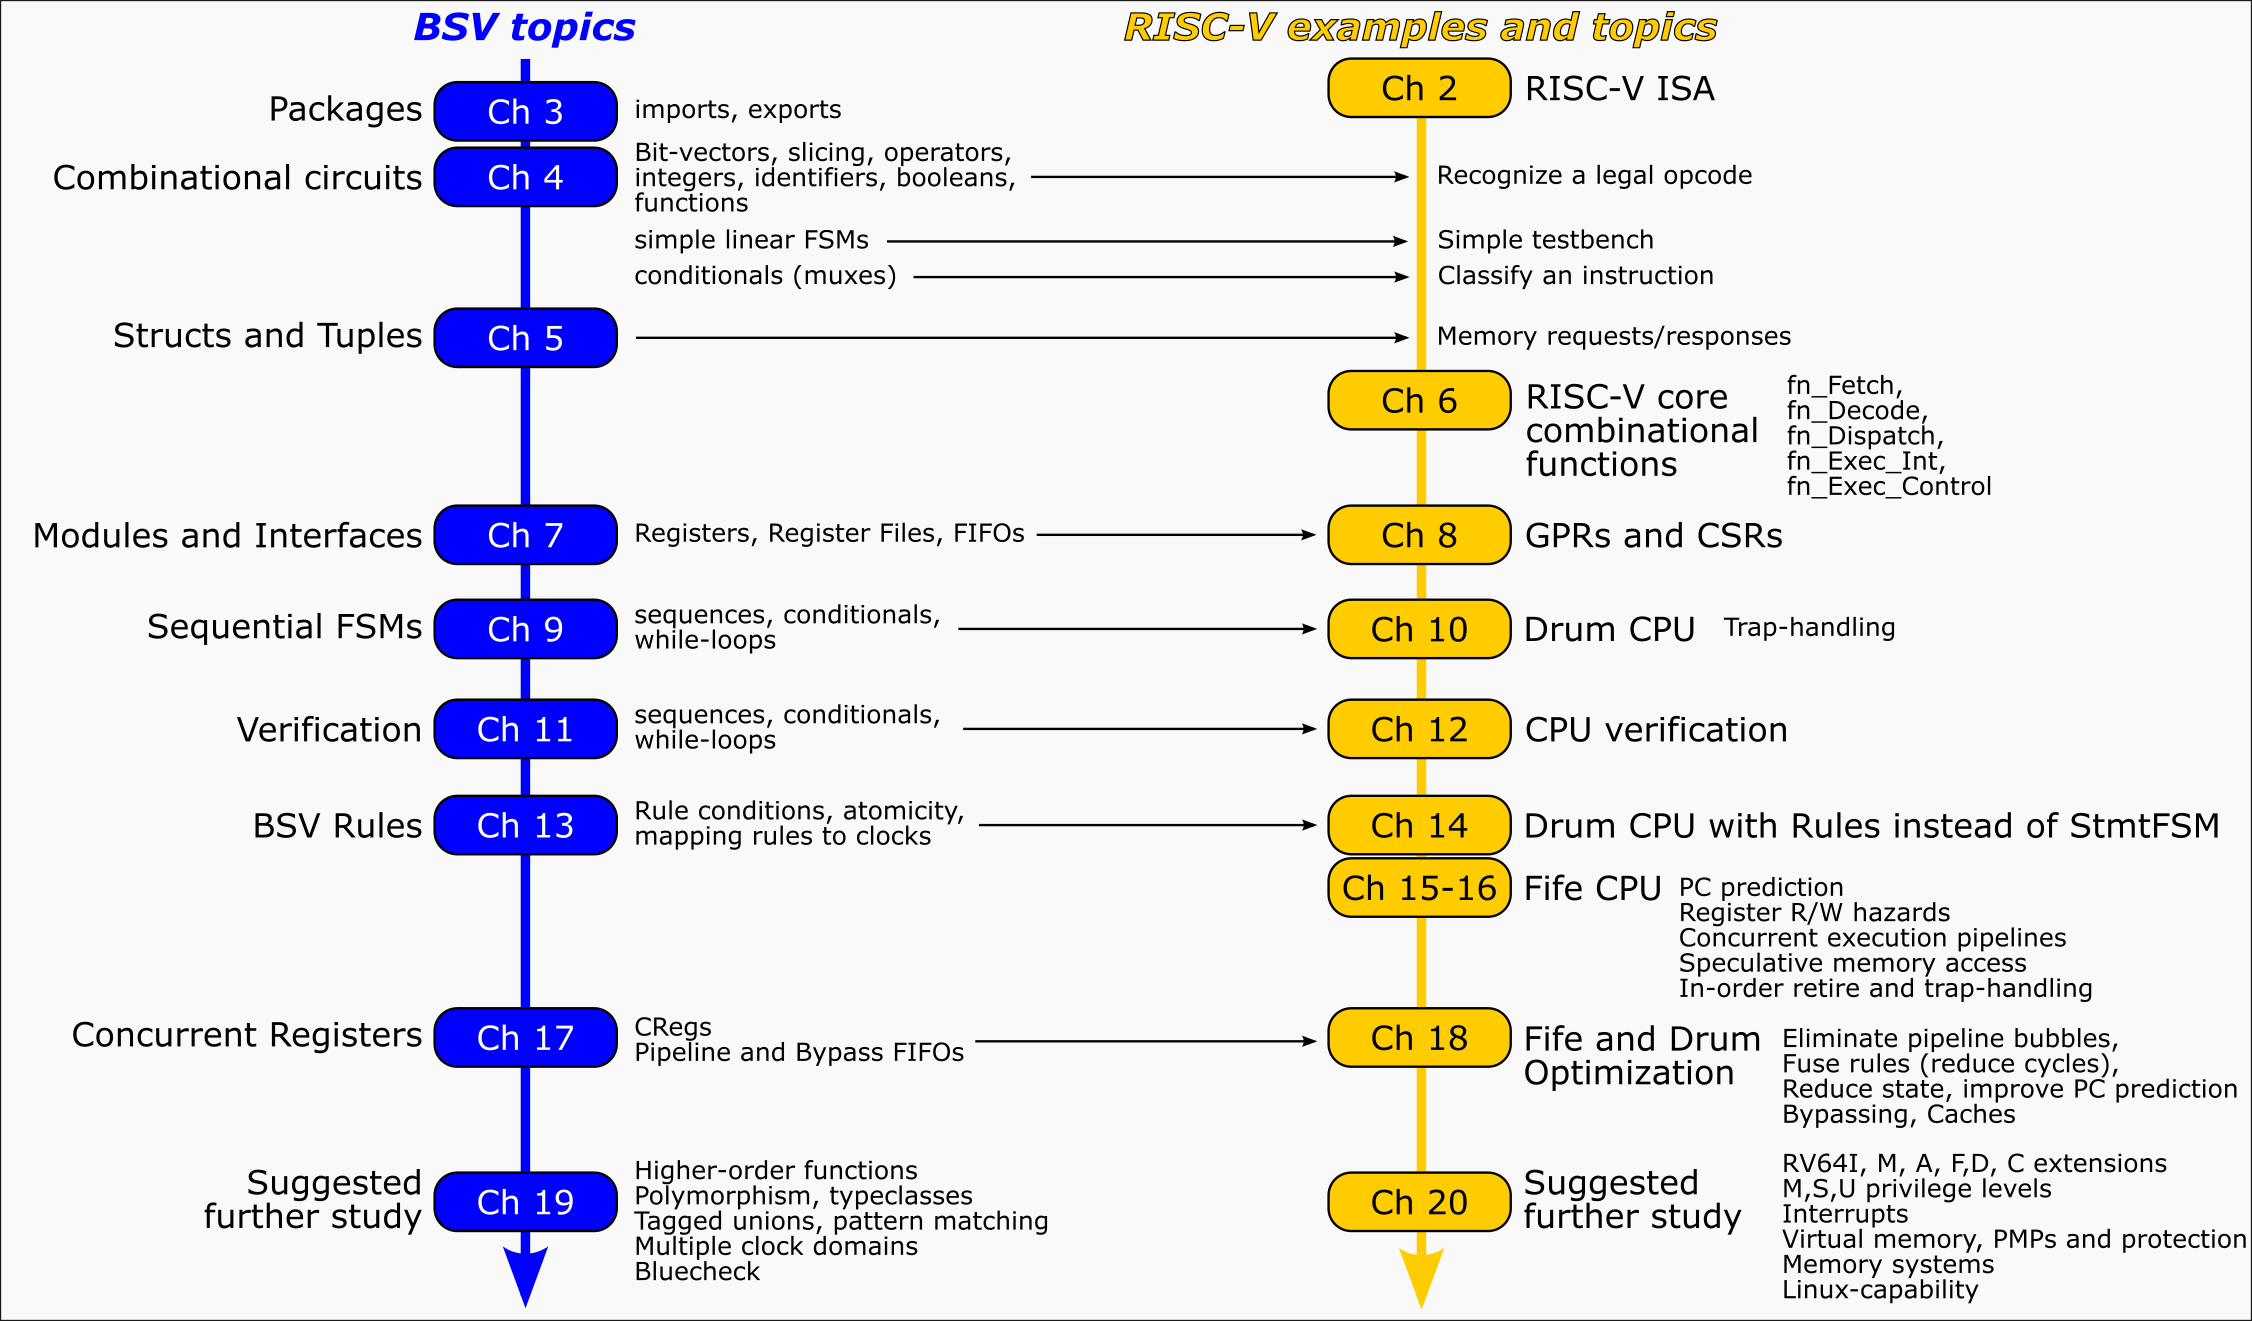
\includegraphics[height=0.825\textheight]{Fig_Chapter_Roadmap}}
\end{center}

\end{frame}

% ================================================================


% ================================================================

\begin{frame}
\frametitle{Table of Contents}

\tableofcontents

\end{frame}

% ****************************************************************

\section{Introduction}

\begin{frame}

\begin{center}
  {\LARGE Introduction}
\end{center}

\end{frame}

% ================================================================

\begin{frame}[fragile]
\frametitle{Functional Correctness {\vs} Performance Correctness}

\footnotesize

{\bf Functional Correctness}:

\vx

\hmmmm \emph{``Does the CPU compute the correct answer?''}

\vxxxx

{\bf Performance Correctness}:

\vx

\hmmmm \emph{``Does the CPU compute the result in an acceptable amount of time?''}

\vxxxx

During CPU verification, typically the initial focus is on functional
correctness.  As the functionality stabilizes, the emphasis moves to
performance correctness.

\end{frame}

% ================================================================

\begin{frame}[fragile]
\frametitle{Complexity of CPU Verification}

\footnotesize

CPU verification is usually much harder than verification of ordinary
(non-CPU) hardware designs because the space of possible inputs is the
space of possible RISC-V programs multiplied by the space of possible
inputs to each RISC-V program.

\vxxxx

\begin{center}
  \begin{minipage}{0.7\textwidth}
    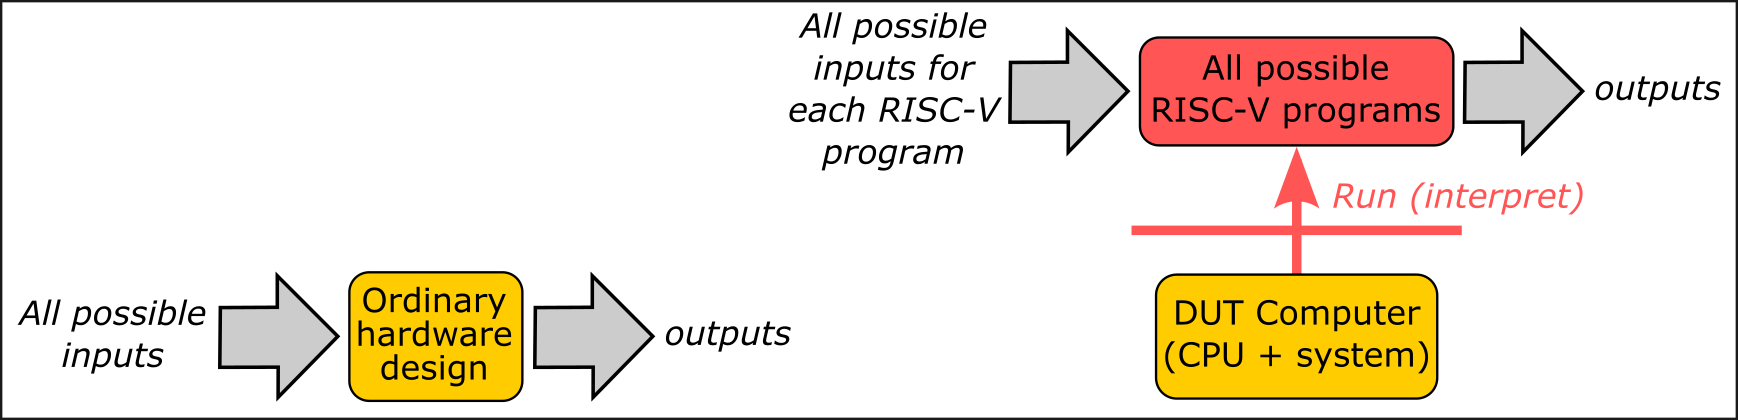
\includegraphics[width=\textwidth]{Fig_CPU_Verif_Complexity}
  \end{minipage}
\end{center}

\end{frame}

% ================================================================

\begin{frame}[fragile]
\frametitle{Determinacy of instruction traces}

\footnotesize

Fortunately, RISC-V program execution is \emph{mostly deterministic},
{\ie} for a given RISC-V program and a given input to the program, the
sequence of instructions executed (its ``instruction trace'') does not
change from one run to the next, nor from one CPU implementation to
another.

\PAUSE{\vxx}

The only sources of non-deteriminism are:

\begin{itemize}
    \item Interrupts (arrive at unpredictable times)

    \vx

    \item Results of a few instructions, such as {\tt rdcycle} and
        {\tt rdtime} (depend on microarchitectural details)

\end{itemize}

\vxx

This allows us to compare the insruction trace of a ``trusted''
execution platform with the instruction trace of the DUT.  Any
divergence indicates a potential bug in the DUT implementation.

\vxxxx

(But, note, we also have to account for non-deteriminacy; we will
discuss that later, under ``asymmetric tandem verification''.)

\end{frame}

% ****************************************************************

\section{Trusted Functional Simulators}

\begin{frame}

\begin{center}
  {\LARGE Trusted Functional Simulators}
\end{center}

\end{frame}

% ================================================================

\begin{frame}[fragile]
\frametitle{Trusted Functional Simulators (``Golden Reference Models'')}

\footnotesize

A Trusted Functional Simulator or Golden Reference Model is a
\emph{simulator} for RISC-V instruction execution, which:

\begin{itemize}

  \item can load and run RISC-V ELF binaries.

  \item at a minimum, produces an \emph{instruction trace}, {\ie} a
      list of PCs of the instructions executed.

      \vx
      By correlating these with the original ELF file, we know the
      instructions executed.

      \vx
      The trace can produce more useful information than just the PCs,
      such as:

      \vx
      \begin{itemize}\scriptsize
          \item the instruction number (sequential number).
          \item the instruction itself (can be verified against the
              ELF file to verify correctness of insruction-fetch)
          \item the new values of any updated registers/CSRs
          \item For Load/Store/AMO instructions, the effective memory
              address for any Load/Store/AMO instruction and the value
              loaded/stored
          \item Trap information, if the instruction trapped
          \item ...
      \end{itemize}
\end{itemize}

\end{frame}

% ================================================================

\begin{frame}[fragile]
\frametitle{Implementations of Trusted Functional Simulators}

\footnotesize

A Trusted Functional Simulator:
\begin{itemize}
  \item is written primarily for clarity and maintainability (for trustworthiness!), \\
      and only secondarily for performance (simulation speed).

  \item is usually written in a software programming language
      (typically C/C++).  This can be run as a standalone program, or
      ``imported'' into an HDL ({\BSV}, Verilog, SystemVerilog, VHDL)
      to run in an HDL simulator.  The purpose of running in an HDL
      simulator is \emph{not} ``cycle-accurary'' (the simulator
      usually is by no means cycle-accurate with any hardware
      implementation), but easy interfacing to other system hardware
      components.

  \item is sometimes written in an HDL.  Again, the purpose of running
      in an HDL simulator is \emph{not} ``cycle-accurary'' (simulator
      ``cycles'' may have no relationship to any hardware
      implementation), but easy interfacing to other system hardware
      components.

  \item is sometimes written in a \emph{synthesizable} HDL ({\BSV},
      Verilog, SystemVerilog, VHDL), in chich case it can be run on an
      FPGA, at potentially much greater speed than a software
      simulator.

      If run an FPGA, one has to provide some means to record the
      instruction trace on a host machine.

\end{itemize}

\end{frame}

% ================================================================

\begin{frame}[fragile]
\frametitle{Trusted Functional Simulators: customizability and speed}

\footnotesize

Additional desirable properties of a trusted functional simulator:
\begin{itemize}

  \item \emph{Configurability/Customizability}: Ability to configure
    it for a particular RISC-V ISA: RV32I vs RV64I; optional M, A, F,
    D, C ISA extensions; optional M,S,U privilege levels; optional
    Sv32/Sv39/Sv48/Sv57 virtual memory schemes; optional multi-hart
    (multi-core); ...

    \vx

    This enables the trusted functional simulator to be used for
    verification of different RISC-V hardware implementations, each of
    which typically makes specific choices amongst these opions.

    \vx

    Configurability/Customizability 

    \vx

    For verifying RISC-V implementations that implement custom ISA
    extensions, the trusted functional simulator needs to be
    customizable also to be able to execute these extensions.

    \vx

    Configurability/Customizability can be:

    \begin{itemize}\scriptsize

      \item Static: recompile and rebuild a version of the simulator
        for a given set of option choices

      \item Dynamic: a single simulator executable conforms to a given
        set of option choices specified in an input file.

    \end{itemize}

  \vxx

  \item \emph{Simulation Speed}: Ability to boot and run an operating
    system ({\eg} Linux) and applications within the OS.  Ability to
    exploit multiple cores in the host computer for greater speed.

    \vx
    Trusted functional simulators can typically boot Linux in minutes,
    sometimes in seconds.  An HDL simulation of an actual RISC-V
    implementation can take days to simulate to the same point.

\end{itemize}

\end{frame}

% ================================================================

\begin{frame}[fragile]
\frametitle{Existing Trusted Functional Simulators: Free and Open-source}

\footnotesize

\begin{minipage}{0.25\textwidth}
  \emph{Spike}

  \vx

  The most famous and widely used trusted functional simulator.
\end{minipage}
\hfill\fbox{
  \begin{minipage}{0.7\textwidth}
    \begin{itemize}

      \item Continuously available since the earliest days of RISC-V.
        Continuously maintained, at high quality, up-to-date with all
        the latest ISA extensions.

      \item Written in C/C++. \\
      Fast (approx. 50-100 MIPS).

      \item Available at: \url{https://github.com/riscv-software-src/riscv-isa-sim}

    \end{itemize}
  \end{minipage}
}

\vx

\begin{minipage}{0.25\textwidth}

  \emph{Sail RISC-V Formal Model}

  \vx

  A little less famous (to date), but equally important.
\end{minipage}
\hfill\fbox{
  \begin{minipage}{0.7\textwidth}
    \begin{itemize}

      \item The ``official'' formal specification for RISC-V, {\ie} the
        official definition of the semantics of the RISC-V ISA (a peer of
        the the textual documents for Unprivileged Spec, Privileged Spec,
        {\etc}).

        \vx

        People who do \emph{formal verification} of RISC-V CPU
        implementations and compilers use this model as the reference
        for proving correctness.

      \item Written in the Sail formal specification language.  Compiled
        by the Sail compiler into an executable under Linux, MacOS, ... \\
        Reasonably fast (approx. 10-20 MIPS).

      \item Available at: \url{https://github.com/riscv/sail-riscv}
    \end{itemize}
  \end{minipage}
}

\end{frame}

% ================================================================

\begin{frame}[fragile]
\frametitle{Other Functional Simulators}

\footnotesize

\begin{minipage}{0.2\textwidth}
  \emph{Qemu}

  \vx

  Widely used.
\end{minipage}
\hm\fbox{
  \begin{minipage}{0.73\textwidth}
    \begin{itemize}

      \item Prioritizes ability to model full systems (CPU,memory,
        devices), for RISC-V software development.

      \item Prioritizes extremely high speed for software development,
        exploiting JIT (Just-In-Time) dynamic compilation. \\
        Very fast (approx. 1 GIPS).

      \item Free, open-source.
    \end{itemize}
  \end{minipage}
}

\vxx


There are probably many functional simulators within many companies in
the RISC-V verification ecosystem, which may not be known
publicly. Two of them are:

\vx

\begin{minipage}{0.2\textwidth}
  \emph{Synopsys ImperasDV}

  \vx

  From Synopysis.

\end{minipage}
\hm\fbox{
  \begin{minipage}{0.7\textwidth}
    \begin{itemize}

      \item The simulator was originally a product of the company
          Imperas, which was aquired by Synopsys in 2023.

      \vx

      \item Imperas' simulator and modeling components are being
          integrated into Synopsys' VCS simulation and DV (Design for
          Verification) suites.

    \end{itemize}
  \end{minipage}
}

\vxx

\begin{minipage}{0.2\textwidth}
  \emph{Cissr}

  \vx

  From Bluespec, Inc.
\end{minipage}
\hm\fbox{
  \begin{minipage}{0.7\textwidth}
    \begin{itemize}

      \item Can model caches, multi-hart, and some devices.

      \item Fast (speed compareable to Spike).

    \end{itemize}
  \end{minipage}
}

\end{frame}

% ****************************************************************

\section{Test programs}

\begin{frame}

\begin{center}
  {\LARGE Test programs}
\end{center}

\end{frame}

% ================================================================

\begin{frame}[fragile]
\frametitle{Test programs}

\footnotesize

CPU verification involves verifying correct behavior over a very large suite of test programs.

\begin{itemize}

  \item \emph{Standard ISA Tests}: RVI (RISC-V International)
        maintains a set of several hundred standardized tests.  These
        are small test programs, written in RISC-V Assembly Language,
        organized by ISA extension: RV32I, RV64I, A, M, F, D and C
        extensions, Machine/Supervisor/User mode, {\etc}

        Available at: \url{https://github.com/riscv-software-src/riscv-tests}

  \vx

  \item \emph{ACTs}: RVI (RISC-V International) is developing a set of
        tests called ACTs (Architecture Compatibility Tests).  Each
        test is a RISC-V program that runs and produces a final
        ``signature'', which is a reliable hash of the final state
        (PC, registers, CSRs, memory, {\etc}).  Over time, these will
        become the official ``certification suite'' for RISC-V.

        \begin{tabbing}
        \hmm \= \url{https://wiki.riscv.org/pages/viewpage.action?pageId=49872986} \\
             \> \url{https://github.com/riscv-non-isa/riscv-arch-test} \\
             \> \url{https://riscof.readthedocs.io/en/stable/}
        \end{tabbing}

  \vx

  \item \emph{riscv-dv}: developed initially at Google; subsequent
        stewardship by the ChipsAlliance non-profit group.  These
        tests generate ``random'' RISC-V programs (constrained to a
        specified ISA subset), run the program on a candidate
        implementation which should generate a trace, and compare
        against a trace from a trusted functional simulator:

        \begin{tabbing}
        \hmm \= \url{https://github.com/chipsalliance/riscv-dv}
        \end{tabbing}

\end{itemize}

\vx

In addition, most organizations maintain their own collection of test
programs and ``regression suites'' (programs that previously surfaced
a bug in some implementation, which are continuously re-run to ensure
that the bug has not resurfaced due to more recent changes).

\end{frame}

% ****************************************************************

\section{Levels of Assurance}

\begin{frame}

\begin{center}
  {\LARGE Levels of Assurance}
\end{center}

\end{frame}

% ================================================================

\begin{frame}
\frametitle{Levels of Assurance}

\footnotesize

\begin{minipage}{0.28\textwidth}

  The ``gold standard'' for assurance that a design is fully correct
  (on all possible inputs) is \emph{Formal Verification}.

  \vx

  This is a very difficult problem, and is still aspirational (there
  are some recent research successes, and the capability improves
  steadily).

  \vxx

  In the meanwhile, we have been doing traditional HW verification.  

\end{minipage}
\hfill
\begin{minipage}{0.7\textwidth}
  \includegraphics[width=\textwidth]{Fig_Levels_of_Assurance}
\end{minipage}

\vxxxx

``\emph{Coverage}'' is a quantifiable measure of how partial/full is
the assurance of correctness:

\begin{itemize}\scriptsize
  \item How many/what fraction of possible inputs are in the suite of test programs?

  \item What fraction of the source code lines in the design have been
        exercised by the suite of test programs?
\end{itemize}
Obviously, the higher these measures, the higher the level of assurance.

\end{frame}

% ================================================================

\begin{frame}[fragile]
\frametitle{Levels of Assurance}

\footnotesize

Here is a sequence of testing regimes with increasing simulation times
but also increasing levels of assurance of the correctness of our CPU
implementation:

\vxx

\begin{itemize}
 \item Run all ``Standard ISA tests'' mentioned.

 \item Run the ACTs and riscv-dv test suites.

 \item Run a small operating system (such as FreeRTOS or Zephyr).

       This will check correct handling of timer interrupts, and
       possibly memory maps and physical memory protection (PMPs).

 \item Boot the kernel of a full-service operating systsem (such as the Linux kernel).

 \item Run a standard distribution a full-service operating systsem
       (such as Debian Linux or Ubuntu Linux), {\ie} the OS kernel
       \emph{plus} the pre-load of all the applications and service
       programs that come with distribution (including block devices
       and networking).  Run applications under the OS.

\end{itemize}

\vxx

The latter items are often executed on FPGA because simulation speed may be too slow.

\end{frame}

% ****************************************************************

\section{Tandem Verification}

\begin{frame}

\begin{center}
  {\LARGE Tandem Verification}
\end{center}

\end{frame}

% ================================================================

\begin{frame}[fragile]
\frametitle{Symmetric Tandem Verification}

\footnotesize

\begin{minipage}{0.6\textwidth}
  \includegraphics[width=\textwidth]{Fig_tandem_verification}
\end{minipage}
\hfill
\begin{minipage}{0.38\textwidth}
  Run a RISC-V binary (ELF file) on two RISC-V implementations, both
  configured for exactly the same RISC-V ISA.  The times taken to
  execute the program may be different.

  \vx

  Usually: one is a trusted functional simulator, the other is the DUT.

  \vx

  Each side produces an \emph{instruction trace}, which we compare for equivalence.

  \vx

  Divergence implies a likely bug in the DUT implemenetation.

\end{minipage}

\vx

\begin{itemize}
  \item At a minimum, the traces specify the sequence of PCs encountered during execution.

        More convenient: traces also specify instruction number, the
        instruction, updates to registers and CSRs, effective address
        in memory for Load/Store/AMO, value loaded/stored for
        Load/Store/AMO, ...

  \item Complication: non-determinism (interrupts, reading
      uninitialized memory, Store-Conditional success/failure, ...).

  \item Complication: modeling the DUT's devices (MMIO) in the reference simulator.

\end{itemize}

\end{frame}

% ================================================================

\begin{frame}[fragile]
\frametitle{Symmetric Tandem Verification: notes}

\footnotesize

\begin{itemize}
  \item Trace outputs can get very large (gigabytes).

  \item ``Offline comparison'': Run the two simulators independently
      and record the output traces.  Separately, compare the traces.

  \item ``Online comparison'': Run the two simulators concurrently (as
      two concurrent processes);

      feed the trace outputs to the comparator running as another
      process that consumes both traces as they are produced.

      Nno need to record the traces, and can stop simulation as soon
      as divergence is detected.

  \item Since the trusted simulator's trace will be the same on
      repeated runs, it can be recorded once and just replayed into
      the (offline or online) comparator.

  \PAUSE{\vxx}

  \item Simulation time and trace sizes can be reduced if the trusted
     simulator and the DUT have ``snapshot'' capability:

     \begin{itemize}\scriptsize

       \item Run the trusted simulator (fast) up to instruction N
         ({\eg} 100 million), then record a snapshot of the entire
         architectural state (all registers, CSRs, memory).

       \item Pre-load the DUT's entire architecture state with the
         snapshot, then resume execution, thereby avoiding simullation
         time for executing the first N instructions.

     \end{itemize}

\end{itemize}

\end{frame}

% ================================================================

\begin{frame}[fragile]
\frametitle{Asymmetric and ``full system'' Tandem Verification (1/2)}

\footnotesize

If we can modify the trusted simulator to run in ``verification
mode'', then Tandem Verification can handle non-determinism and
devices (MMIO).  \hmm (Details on next slide.)

\vxx

\begin{center}
\begin{minipage}{0.7\textwidth}
  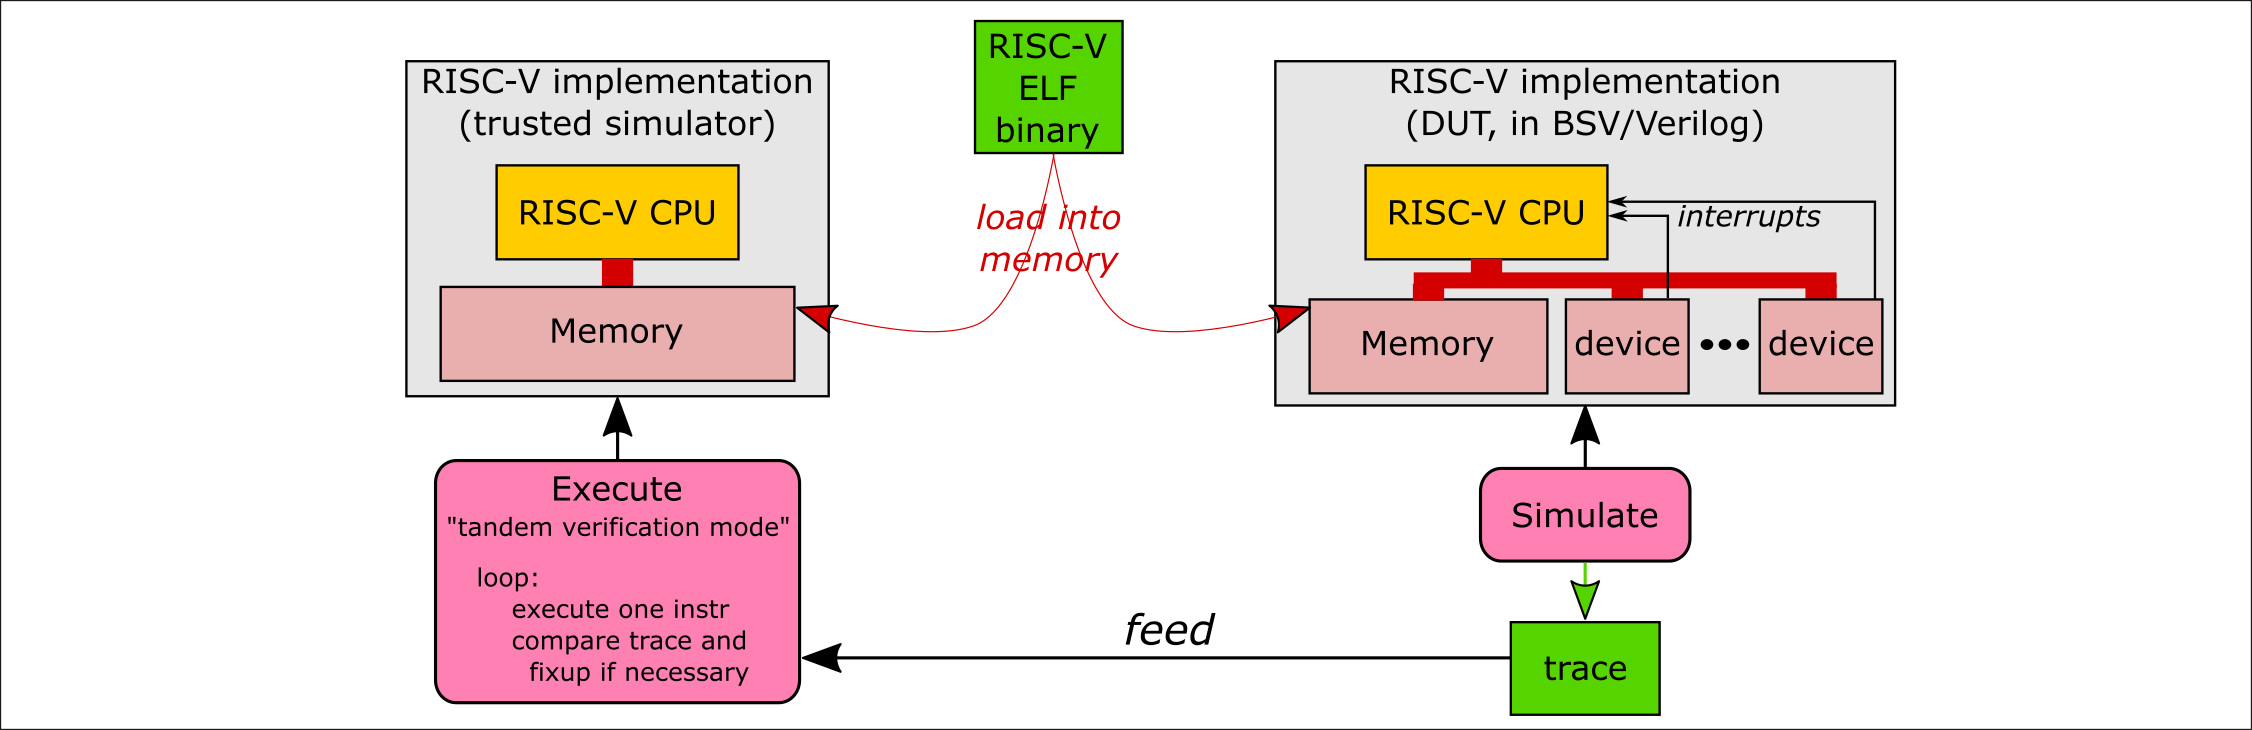
\includegraphics[width=\textwidth]{Fig_tandem_verification_II}
\end{minipage}
\end{center}

\end{frame}

% ================================================================

\begin{frame}[fragile]
\frametitle{Asymmetric and ``full system'' Tandem Verification (2/2)}

\footnotesize

The trusted simulator consumes the trace from the DUT simulation
either in real time (online) or from a recording (offline) and,
normally, compares each instruction from the trace with its own
behavior (as in symmetric tandem verification).

\begin{itemize}

  \item \emph{Non-determinism: interrupts}: the DUT trace should
      include interrupt events:
      \begin{itemize}\scriptsize

        \item[(a)] when a bit in CSR MIP changes state ($0 \rightarrow
            1$ and $1 \rightarrow 0$), and

        \item[(b)] when an interrupt is actually taken (responding to a 1 bits in MIP).

      \end{itemize}

      For (a), the trusted simulator records the same change in its
      CSR MIP.

      For (b), the trusted simulator checks that it is legal to take
      this interrupt at this point in the trace and, if so, also takes
      the same interrupt at this point.

  \item \emph{Non-determinism: Store-conditional success/fail result,
      {\tt rdtime} and {\tt rdcycle} instructions}: the DUT takes the
      value from the trace instead of its own.

  \item \emph{Non-determinism: Reading uninitialized memory}:
      if the trusted simulator and the DUT disagree on a load-value,
      it could be because of uninitialized memory (and memory was not
      initialized identically in the two simulators).

      The verifier can issue a warning message, take the load-value
      from the DUT trace as the loaded value, and proceed.

  \item \emph{Device (MMIO) Loads}: the trusted simulator takes the
      loaded value (or load exception) from the trace.

  \item \emph{Device (MMIO) Stores}: the trusted simulator discards
      the stored value.  If the trace indicates that the store
      response is an exception, the trusted simulator takes the same
      exception.

\end{itemize}

\end{frame}

% ****************************************************************

\section{Testbench for Drum and Fife}

\begin{frame}

\begin{center}
  {\LARGE Testbench for Drum and Fife}
\end{center}

\end{frame}

% ================================================================

\begin{frame}[fragile]
\frametitle{Testbench for Drum and Fife (1/2)}

\footnotesize

We use exactly the same testbench for Drum and Fife (discussion on
next slide):

\vxx

\includegraphics[width=\textwidth]{Fig_CPU_Simulation}

\end{frame}

% ================================================================

\begin{frame}[fragile]
\frametitle{Testbench for Drum and Fife (2/2)}

\footnotesize

\begin{itemize}
  \item {\tt mkMems\_Devices} models everything outside the CPU (memory and devices).

      It is actually implemented in C and imported into a {\BSV}
      wrapper using a standard mechanism provided by {\BSV}.

  \vx

  \item {\tt mkTop} mostly just instantiates {\tt mkCPU} (Drum or
      Fife) and {\tt mkMems\_Devices}, passing the former's memory
      interfaces into the latter.

  \vx

  \item {\tt mkTop} only performs the following:

      \begin{itemize}
        \item invokes the CPU's {\tt init} method once, at startup, to
            provide the CPU with the initial value of the PC (from
            which it should start fetching).

        \vx

        \item continually (on every clock) relays the value of real
            time from {\tt mkMems\_Devices} to the CPU, which places
            it in its CSR TIME.  This is the value read by the {\tt
            rdtime} instruction.

      \end{itemize}

  \item {\tt mkMems\_Devices} continually dequeues memory requests
      from the CPU using its {\tt fo\_IMem\_req} and {\tt
      fo\_DMem\_req} methods.  For each request it invokes C code to
      compute a response and returns it to the CPU using the using its
      {\tt fi\_IMem\_rsp} and {\tt fi\_DMem\_rsp} methods.

      The C code internally models memory as an ordinary C array of
      bytes, and it contains a model of a standard 16550 UART for
      character I/O.

\end{itemize}

\end{frame}

% ****************************************************************

\section{Final Comments}

\begin{frame}[fragile]
\frametitle{Final comments on RISC-V Verification}

\footnotesize

\begin{itemize}

  \item The functional verification question is:

        \hmm
        \begin{minipage}{0.9\textwidth}
            \emph{Does this CPU implementation always produce the
            correct answer, for any RISC-V program that we load into
            its memory?}
        \end{minipage}

        \vx

        The performance verification question is:

        \hmm
        \begin{minipage}{0.9\textwidth}

            \emph{Does this CPU implementation produce its answer in
            the expected time, for any RISC-V program that we load
            into its memory?}

        \end{minipage}

        \vx

        This chapter is only about functional verification

  \vx

  \item Formal verification is the gold standard for functional
        verification, but the technology is not yet ready for
        production use.  With today's technology it is routinely used
        for verifying simple properties and verifiying components.

  \vx

  \item Until then, verification is done by running test programs and
        comparing program outputs and instruction traces with
        corresponding outputs and traces from a trusted functional
        simulator.

        \vx

        This comparison is called ``tandem verification'', which can
        be online or offline, symmetric or asymmetric (the latter has
        advantages in dealing with non-determinism and devices (MMIO).

        \vx

        ``Coverage metrics'' quantify the level of assurance.
\end{itemize}

\end{frame}

% ****************************************************************

% -*- mode: fundamental -*-

% Slides accompanying "Learn RISC-V CPU Implementation and BSV" book
% Copyright (c) 2024 Rishiyur S. Nikhil, All Rights Reserved

% This is a postamble shared by all the slide decks

% ================================================================

\begin{frame}

\begin{center}
  {\LARGE End}
\end{center}

\end{frame}

% ================================================================


% ****************************************************************

\end{document}

% ****************************************************************
